\chapter{Fallstudie}
\label{chap:evaluation}

Nachdem die verschiedenen Konsistenzregeln aufgestellt und implementiert wurden, soll nun die Benutzbarkeit und die Erweiterbarkeit des Tools gezeigt werden.
Dafür wird in diesem Kapitel eine beispielhafte Anwendung des Tools, aus Sicht des Benutzers, durchgeführt (Abschnitt 1) und anschließend eine neue Regel, aus Sicht des Entwicklers, implementiert (Abschnitt 2).

\section{Anwendung am Beispiel einer Pizzabestellung}

In ihrer Arbeit haben \cite{Schoen} für die Einführung in BROS das Beispiel einer Pizzabestellung erstellt.
Das dort gegebene BPMN-Modell wird als Grundlage genutzt, um ein neues BROS-Modell zu erstellen, und die Konsistenz mit Hilfe des neu entwickelten Tools zu überprüfen.
Die Modelle werden zu diesem Zweck neu in bpmn.io und FRaMED.io modelliert, um sie automatisiert überprüfen zu können.
Nachdem ein konsistentes BROS-Modell entwickelt wurde, wird die Benutzbarkeit des Tools diskutiert.

\begin{figure}
    \centering
    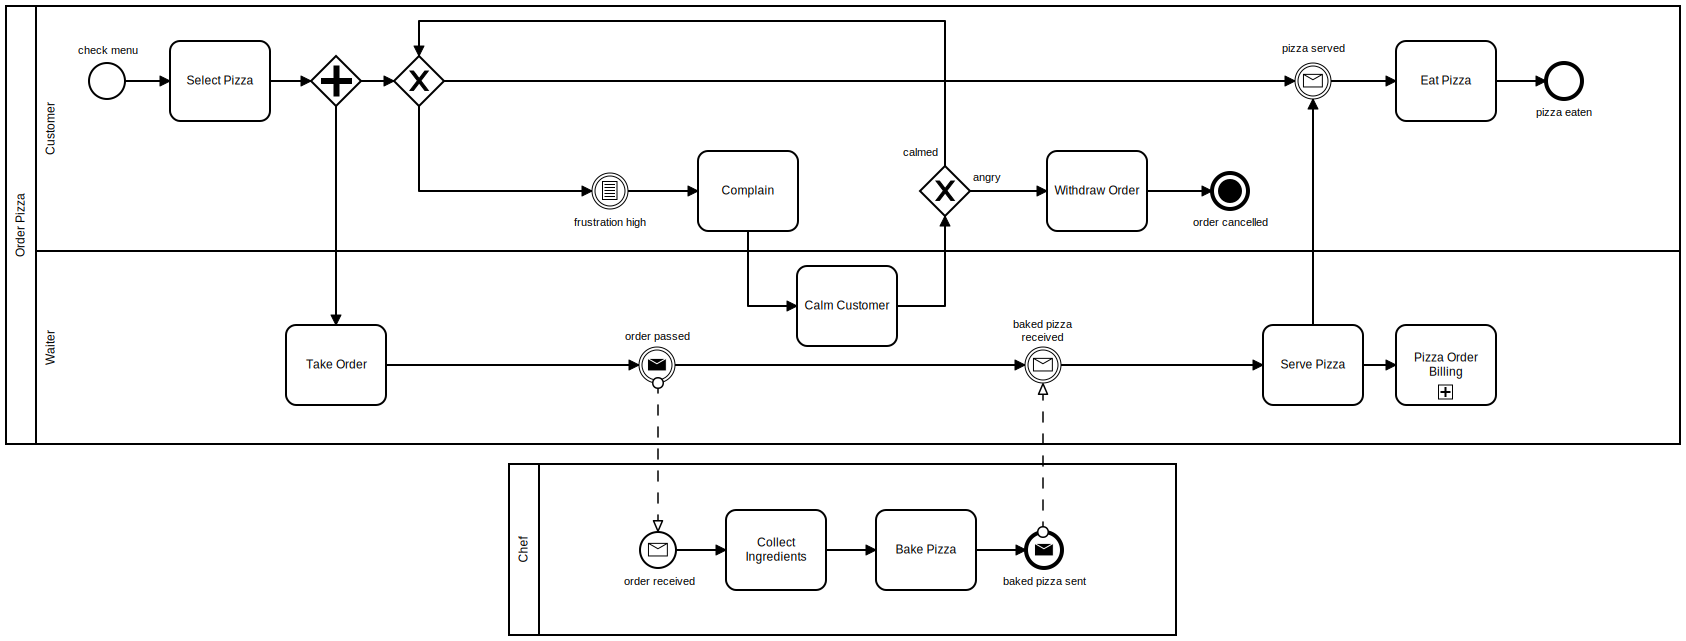
\includegraphics[width=\textwidth,keepaspectratio]{../images/example/bpmn.pdf}%
    \caption{BPMN-Modell der Pizzabestellung}%
    \label{fig:pizzaBpmn}
\end{figure}

In dem Geschäftsprozess der Pizzabestellung gibt es drei Teilnehmer, die in \cref{fig:pizzaBpmn} zu sehen sind.
Der erste Teilnehmer ist der \emph{Kunde}.
Dieser startet den Prozess indem er eine Bestellung aufgibt.
Die Bestellung wird von dem \emph{Kellner} aufgenommen und an den \emph{Koch} weiter gereicht.
Falls, während die Bestellung von dem Koch bearbeitet wird, die Bestellung länger benötigt als gewöhnlich, kann sich der Kunde bei dem Kellner beschweren, dessen Aufgabe dann das beruhigen des Kunden ist.
Sollte dies nicht erfolgreich sein, kann der Kunde seine Bestellung zurücknehmen, was den Prozess vorzeitig beendet.
Nachdem der Koch die Pizza fertig zubereitet hat, übergibt er sie wieder dem Kellner, der die Bestellung dem Kunden überreicht.
Anschließend erstellt der Kellner noch die Rechnung für den Kunden.
Sobald der Kunde die Pizza gegessen hat, ist der Prozess beendet.

\begin{figure}
    \centering
    \includegraphics[width=\textwidth,keepaspectratio]{../images/example/bros-rule1.png}%
    \caption{Entwurf für das BROS-Modell der Pizzabestellung}%
    \label{fig:pizzaBros1}
\end{figure}

Für dieses BPMN-Modell kann nun ein dazu passendes BROS-Modell entworfen werden (vgl. \cref{fig:pizzaBros1}).
Aus dem Prozess lassen sich vier verschiedene Entitäten entnehmen.
Dies sind \emph{Bestellung}, \emph{Pizza}, \emph{Gast} und \emph{Mitarbeiter}, welche als NaturalType modelliert werden.
Der gesamte Prozess wird mit der Scene \emph{Pizzabestellung} abgebildet.
Die drei Teilnehmer aus dem BPMN-Modell werden mit Rollen innerhalb der Scene übersetzt, die mit Events verbunden sind.
Der Ablauf einer Beschwerde von einem Kunden, wird mit einer eigenständigen Scene modelliert, die zwei verschiedene ReturnEvents besitzt.
Diese stellen den Ausgang des Beschwichtigungsversuches durch den Kellner dar.

Nachdem beide Modelle erstellt wurden, kann die Konsistenzprüfung mit dem Tool erfolgen.
Dafür werden die beiden gespeicherten Dateien, mittels Drag'n'Drop in das Benutzerinterface gezogen, wodurch die Prüfung automatisch startet.
Bei der Überprüfung konnten die Regeln 18 mal angewendet werden und es wurden 12 positive Konsistenzmeldungen zurückgegeben.
Damit sind in dem BROS-Modell 6 Konsistenzprobleme aufgetreten.
Die davon betroffenen Regeln sind die Regeln 1, 3, 4, 5 und 6.

\begin{figure}[H]
    \centering
     \includegraphics[width=0.95\textwidth,keepaspectratio]{../images/example/error1.png}%
    \caption{Regelverstoß 1: Kein BROS-Element gefunden}%
    \label{fig:error1}
\end{figure}

Der erste Regelverstoß (vgl. \cref{fig:error1}) hat seinen Ursprung in der Regel 1 und besagt, dass für den Bpmn-Prozess ``Order Pizza'' kein entsprechendes BROS-Element gefunden werden konnte.
Dies liegt an dem Namensunterschied gegenüber der BROS-Scene, die ``Pizzabestellung'' heißt.
Ein derartiges Konsistenzproblem lässt sich auf zwei unterschiedlichen Wegen lösen.
Zum einen kann ein Predefined Matching zwischen dem BPMN-Prozess und der BROS-Scene erstellt werden.
Dazu kann der BPMN-Prozess mit einem Klick auf die ID markiert werden.
Die BROS-Scene ist unter dem Reiter \emph{BROS matching} auffindbar und kann mit einem Klick ebenfalls markiert werden.
In dem Dialog am unterem Bildschirmrand, kann nun das Matching hinzugefügt werden, wodurch die Überprüfung erneut durchgeführt wird.
Um die Konsistenz auch für zukünftige Modelle des Geschäftsprozesses zu erhalten, kann die BROS-Scene auch umbenannt werden.

\begin{figure}[H]
    \centering
     \includegraphics[width=0.95\textwidth,keepaspectratio]{../images/example/error2.png}%
    \caption{Regelverstoß 2: Endelemente der Events sind unterschiedlich}%
    \label{fig:error2}
\end{figure}

Regel 4 ist die Ursache für das zweite Konsistenzproblem.
Es besagt, dass das BPMN-EndEvent ``pizza eaten'' zwar ein Matching mit dem BROS-ReturnEvent ``Pizza  eaten'' aufweist, aber beide Elemente unterschiedliche Teilprozesse beenden (vgl. \cref{fig:error2}).
Dies liegt an der fehlenden Zuordnung des BPMN-Prozesses ``Order Pizza'' und der BROS-Scene ``Pizzabestellung''.
Da diese Zuordnung schon mit dem Lösen des ersten Regelverstoßes behoben wurde, ist keine weitere Änderung notwendig.
Nachdem die BROS-Scene zu ``OrderPizza'' umbenannt (vgl. \cref{fig:pizzaBros3}) wurde, kann die Konsistenzprüfung mit dem Laden der neuen Datei wiederholt werden.

\begin{figure}[H]
    \centering
    \includegraphics[width=0.95\textwidth,keepaspectratio]{../images/example/error3.png}%
    \caption{Regelverstoß 3: Kein BROS-Element gefunden}%
    \label{fig:error3}
\end{figure}

Das dritte Problem stammt von der Regel 3 und beschreibt, dass zu dem BPMN-Termination\-Event ``order cancelled'' kein passendes BROS-ReturnEvent gefunden wurde (vgl. \cref{fig:error3}).
Dieses Problem stammt von dem vergessenen BROS-ReturnEvent.
Es kann leicht behoben werden, indem zu der BROS-Scene noch ein weiteres BROS-ReturnEvent mit dem Namen ``order cancelled'' hinzugefügt wird (vgl. \cref{fig:pizzaBros4}). 
Dabei erhöht sich auch die Anzahl der zutreffenden Regeln um eins auf 19, da ein weiteres BROS-Event existiert, das mit Regel 6 überprüft werden muss.

\begin{figure}[H]
    \centering
    \includegraphics[width=0.95\textwidth,keepaspectratio]{../images/example/error4.png}%
    \caption{Regelverstoß 4: Endelemente der Events sind unterschiedlich}%
    \label{fig:error4}
\end{figure}

Für das vierte Konsistenzproblem ist Regel 4 verantwortlich.
Es besagt, dass für das BPMN-EndEvent ``baked pizza send'' zwar ein BROS-Event im Matching gefunden werden konnte, aber die Elemente, die von den Events beendet werden, unterschiedlich sind (vgl. \cref{fig:error4}).
Das BPMN-EndEvent beendet die BPMN-Swimlane für den Koch, das BROS-Event hingegen beendet nichts.
Dies liegt an einer fehlerhaften Verknüpfung der BROS-Event.
Momentan wird die BROS-Rolle ``TastyPizza'' von dem BROS-Event ``baked pizza send'' erzeugt, was allerdings falsch ist.
Für das Erzeugen dieser BROS-Rolle ist das BROS-Event ``pizza served'' verantwortlich.
Das BROS-Event ``baked pizza send'' wird hingegen mit einer BROS-DestroyRelation mit der BROS-Rolle des Koches vebunden, wie in \cref{fig:pizzaBros5} zu sehen ist.

\begin{figure}[H]
    \centering
    \includegraphics[width=0.95\textwidth,keepaspectratio]{../images/example/error5.png}%
    \caption{Regelverstoß 5: Kein BROS-Element gefunden}%
    \label{fig:error5}
\end{figure}

Der vorletzte Regelverstoß basiert auf der Regel 5 und ist trivial zu lösen.
Er beschreibt, dass zu dem BPMN-StartEvent ``check menu'' kein passendes BROS-Event mit einer BROS-CreateRelation zu der BROS-Scene ``OrderPizza'' existiert (vgl. \cref{fig:error5}).
Dieses BROS-Event wurde im bisherigen BROS-Model vergessen.
Zum Lösen des Konsistenzproblems, muss ein BROS-Event mit dem Namen ``check menu'' und der dazugehörigen BROS-CreateRelation hinzugefügt werden (vgl. \cref{fig:pizzaBros6}).

\begin{figure}[H]
    \centering
    \includegraphics[width=0.95\textwidth,keepaspectratio]{../images/example/error6.png}%
    \caption{Regelverstoß 6: Kein BPMN-Element gefunden}%
    \label{fig:error6}
\end{figure}

Anschließend bleibt nur noch ein Konsistenzproblem übrig.
Dieses besagt, dass ein Verstoß gegen Regel 6 vorliegt, indem zu dem BROS-Event ``pizza lost'' kein passendes BPMN-Element gefunden wurde (vgl. \cref{fig:error6}).
Das ist ein Problem, welches sich nicht einfach lösen lässt, da kein passendes BPMN-Element existiert.
Mit dem BROS-Event wurde das Modell um eine neue Funktionalität erweitert, die die Konsistenz verletzt.
Um dieses Problem zu lösen, muss entweder das BROS-Event gelöscht oder das BPMN-Modell angepasst werden.
Wenn das BROS-Event aber erhalten bleiben soll, und es keine Möglichkeit gibt das BPMN-Modell zu ändern, muss dieser Regelverstoß ignoriert werden.

\begin{figure}
    \centering
    \includegraphics[width=\textwidth,keepaspectratio]{../images/example/bros-rule6H.png}%
    \caption{Vollständiges BROS-Modell der Pizzabestellung}%
    \label{fig:pizzaBros6}
\end{figure}

Damit zeigt \cref{fig:pizzaBros6} das vollständige BROS-Modell, das so weit wie möglich mit dem BPMN-Modell konsistent ist.
Dank des Tools konnten viele Konsistenzprobleme gefunden und leicht behoben werden.
Die zu \cref{fig:pizzaBros1} geänderten Modellelemente sind in \cref{fig:pizzaBros6} rot markiert und mit der Fehlernummer annotiert.
Mit der letzten negativen Konsistenzmeldungen des Tools wurde gezeigt, dass ein Regelverstoß absichtlich herbeigeführt werden kann und dies nicht unbedingt einen Fehler darstellt.
Das Tool hat zurzeit keine Möglichkeit mit bewussten Konsistenzproblemen umzugehen.
Hierfür wäre eine Funktion zur manuellen Abstufung der Regelverletzung von einem Fehler zu einer Warnung oder Information hilfreich.

\section{Erweiterbarkeit des Ansatzes}

Bisher wurden nur Regeln in ihre Kotlin-Implementierung überführt, die die Konsistenz von BPMN-Modellen zu BROS-Modellen prüfen.
Da das BROS-Modell gegenüber dem BPMN-Modell angereichert werden kann ist dies auch die häufigste Anwendung.
Allerdings können auch einige Regeln in die andere Richtung überprüft werden.
Um gleichzeitig die Erweiterbarkeit des Ansatzes und der Implementierung zu zeigen, wird \textbf{Regel 6} aus \cref{sec:Konsistenzregeln} hinzugefügt.
Die Regel 6 überprüft, dass zu jedem BROS-Event und BROS-ReturnEvent ein dazugehöriges BPMN-Element existiert. 
Dabei können die BPMN Elemente von den Typen BPMN-Activity, BPMN-Gateway und BPMN-Event sein. 
Der genaue Typ des BPMN-Events ist dabei nicht relevant, es kann sich dabei unter anderem um ein BPMN-StartEvent oder auch ein BPMN-TerminationEvent handeln.

Jede Regel sollte zur besseren Übersicht in eine eigene Datei ausgelagert werden.
Die bereits bestehenden Regeln befinden sich im Package \emph{io.framed.modules}.
Für die Regel 6 wird dafür die Datei \emph{Rule6BrosEvent.kt} erstellt.
Jede Datei enthält eine Funktion, die zum Setup der Regeln ausgeführt wird.
Dies hat die Signatur \emph{fun Context.setupRule6BrosEvent()}.
Damit wird ein Parameter definiert, der den Typ \emph{Context} hat und als Receiver (\emph{this}) genutzt werden kann.
Innerhalb dieser Funktion können nun die Matching- und Verifikations-Funktionen definiert werden.
Die explizite Angabe des \emph{Context}-Receiver-Parameters ist nun nicht mehr nötig, da dies durch die Setup-Funktion an ihre inneren Funktionen propagiert wird. 

Die Matching Regeln zwischen den verschiedenen BPMN-Events und dem BPMN-Gateway wurden im \cref{sec:matching_model_elements} bereits implementiert.
Für die Erweiterung muss damit nur die Matching Regel für BPMN-Activities mittels Name-Matching hinzugefügt werden.
Dabei wird in den generischen Parametern nach BPMN-Activities und BROS-Events gefiltert.
Diese werden mittels ihrer Namen verglichen und bei erfolgreichen Vergleich zum Matching hinzugefügt.
Da BROS-Events und BROS-ReturnEvents unterschiedliche Metamodell Typen haben, muss diese Matching-Regel ein weiteres mal hinzugefügt werden, wobei der generische Parameter für das BROS-Modell auf ein BROS-ReturnEvent gesetzt wird.
Die Implementierung des Lambdas bleibt unverändert.

\begin{lstlisting}[language=Kotlin, caption=Matching Regel zwischen BPMN-Activities und BROS-Events, label=lst:matching_activity_event]
match<BpmnTask, BrosEvent> { bpmn, bros ->
    matchStrings(bpmn.element.name, bros.element.desc)
}
\end{lstlisting}

Nachdem das Matching auf die unterstützten Modellelemente erweitert wurde, kann nun die Verifikationsregel implementiert werden.
Anders als die in \cref{sec:implementaion_consistency_rules} implementierten Regeln, ist Regel 6 von dem BROS-Modell aus gerichtet.
Darum wird nicht die Funktion \emph{verifyBpmn}, sondern die äquivalente Funktion \emph{verifyBros} genutzt.
Im generischen Parameter der Funktion wird nach einem BROS-Event gefiltert.
Innerhalb des Lambdas wird überprüft, ob es ein BPMN-Element im Matching des BROS-Events gibt.
Hier wird zur Vereinfachung des Quellcodes ausgenutzt, dass mit den Matching Regeln keine unzulässigen BROS-Elemente im Matching aufgenommen werden können.
Sollte das Matching mit anderen BROS-Event zu BPMN-Element Regeln erweitert werden, muss im Schleifenkörper eine genauere Überprüfung des BPMN-Element Typs erfolgen.
Analog zu der neuen Matching-Regel muss auch die Verifikationsregel ein weiteres mal mit dem Filter nach BROS-ReturnEvents eingefügt werden.

\begin{lstlisting}[language=Kotlin, caption=Implementierung von Regel 6, label=lst:implementation_rule_6]
verifyBros<BrosEvent> { bros ->
    for (bpmn in bros.matchingElements) {
        if (bpmn.checkType<BpmnElement>()) {
            return@verifyBros Result.match("...", bpmn = bpmn)
        }
    }
    Result.error("...")
}
\end{lstlisting}

Ein Nachteil der \emph{Kotlin/JS} Plattform ist das Fehlen von \emph{Reflections} und \emph{Annotation-Processing} wie in Java bzw. \emph{Kotlin/JVM}.
Aus diesem Grund wird die neu hinzugefügte Setup-Funktion nicht automatisch erkannt und muss manuell registriert werden.
In der Datei \emph{io.framed.modules.Main.kt} existiert eine Liste von Setup-Funktionen, die ausgeführt werden.
Um nun die neue Regel im Tool zu registrieren, wird die Liste um einen neuer Eintrag (\emph{Context::setupRule6BrosEvent}) ergänzt.
Der Aufruf ``::'' auf eine Funktion, gibt eine Funktionsreferenz zurück und erlaubt eine spätere Ausführung.
Die vollständige Implementierung der Regel 6 ist unter \cref{lst:Rule6BrosEvent} zu finden.
